\documentclass[a4paper,11pt,fleqn,oneside,openany]{memoir} 	% Openright aabner kapitler paa hoejresider (openany = vilkaarlig/begge)
%,draft

\usepackage{placeins}
%%%% PAKKER %%%%
% ¤¤ Oversaettelse og tegnsaetning ¤¤ %
\usepackage[utf8]{inputenc}					% Input-indkodning af tegnsaet, dvs. input fra keyboard, tegnoversigt eller andet (UTF8 = Unicode)
\usepackage[T1]{fontenc}					% Output-indkodning af tegnsaet, dvs. printede fonte og tegn (T1 = Type 1 font med support for de fleste europaeiske sprog)
\usepackage{lmodern}
\usepackage[english]{babel}					% Sproglig fremstilling af elementer (figur vs. figure, litteratur vs. bibliography osv.)
\usepackage{ragged2e,anyfontsize}			% Justering af elementer

\usepackage{multicol}

\usepackage{graphicx,wrapfig,lipsum}
\usepackage[newfloat]{minted}
\usepackage{xcolor}
% ¤¤ Figurer og tabeller (floats) ¤¤ %
\usepackage{graphicx} 						% Inkludering af eksterne billeder (JPG, PNG, PDF)
\usepackage{multirow}                		% Fletning af raekker og kolonner (\multicolumn og \multirow)
\usepackage{colortbl} 						% Farver i tabeller (fx \columncolor, \rowcolor og \cellcolor)

\usepackage{float}							% Muliggoer eksakt placering af floats, fx \begin{figure}[H]
\let\newfloat\relax 						% Justering mellem float-pakken og memoir
%\usepackage{eso-pic}						% Tilfoej billedekommandoer paa hver side
%\usepackage{wrapfig}						% Indsaettelse af figurer omsvoebt af tekst 
%\usepackage{multicol}         	        	% Muliggoer tekst i spalter
%\usepackage{rotating}						% Rotation af tekst med \begin{sideways}...\end{sideways}

% ¤¤ Matematik mm. ¤¤
\usepackage{amsmath,amssymb,stmaryrd} 		% Avancerede matematik-udvidelser
\usepackage{mathtools}						% Andre matematik- og tegnudvidelser
\usepackage{textcomp}                 		% Symbol-udvidelser (fx promille-tegn med \textperthousand)
\usepackage[binary-units]{siunitx}						% Flot og konsistent praesentation af tal og enheder med \si{enhed} og \SI{tal}{enhed}
\sisetup{output-decimal-marker = {,}}		% Opsaetning af \SI og decimalseparator
%\usepackage[version=3]{mhchem} 			% Kemi-pakke til flot og let notation af formler, fx \ce{Fe2O3}
%\usepackage{rsphrase}						% Kemi-pakke til RS-saetninger, fx \rsphrase{R1}

% ¤¤ Referencer og kilder ¤¤ %
\usepackage[danish]{varioref}				% Muliggoer bl.a. krydshenvisninger med sidetal (\vref)
\usepackage{natbib}							% Udvidelse med naturvidenskabelige citationsmodeller, herunder Harvard-modellen
%\usepackage{xr}							% Referencer til eksternt dokument med \externaldocument{<NAVN>}
%\usepackage[acronym, toc]{glossaries}					% Terminologi- eller symbolliste (se mere i Lars Madsens Latex-bog)
\usepackage[nomain, acronym, toc, nonumberlist, automake]{glossaries-extra}
\makeglossaries
% \newacronym{gcd}{GCD}{Greatest Common Divisor}

% \newacronym{lcm}{LCM}{Least Common Multiple}

\newacronym{sdr}{SDR}{Software Defined Radio}
\newacronym{iso}{ISO}{International Organisation of Standardisation}


% \newglossaryentry{Software Defined Radio}
% {
%     name=Software Defined Radio,
%     description= {A software defined radio is based on an antenna, a receiver front end and the mixer software run on a processor. The main difference between typical (hardware) radios and Software defined radios is that the signal processing is performed in software instead of on hardware, which requires varying amounts of computing power depending on the sampling rate, as the system is digital instead of analogue. Some of the benefits in space applications include the ability to re-tune or re-purpose the radio through software.}
% }





%\setabbreviationstyle[acronym]{long-short}

% ¤¤ Misc. ¤¤ %

\usepackage{listings}						% Placer kildekode i dokumentet med \begin{lstlisting}...\end{lstlisting}
\usepackage{lipsum}							% Dummy tekst med fx \lipsum[2]
\usepackage[shortlabels]{enumitem}			% Muliggoer enkelt konfiguration af lister (se \setlist nedenfor)
\usepackage{pdfpages}						% Goer det muligt at inkludere pdf-dokumenter med kommandoen \includepdf[pages={x-y}]{fil.pdf}	
\pdfoptionpdfminorversion=6					% Muliggoer inkludering af pdf-dokumenter af version 1.6 og hoejere
\pretolerance=2500 							% Justering af afstand mellem ord (hoejt tal, mindre orddeling og mere luft mellem ord)

% Kommentarer og rettelser med \fxnote. Med 'final' i stedet for 'draft' udloeser hver note en error i den faerdige rapport.
\usepackage[footnote,draft,danish,silent,nomargin]{fixme}		


%%%% BRUGERDEFINEREDE INDSTILLINGER %%%%

% ¤¤ Marginer ¤¤ %
\setlrmarginsandblock{3.5cm}{2.5cm}{*}		% \setlrmarginsandblock{Indbinding}{Kant}{Ratio}
\setulmarginsandblock{2.5cm}{3.0cm}{*}		% \setulmarginsandblock{Top}{Bund}{Ratio}
\checkandfixthelayout 						% Oversaetter vaerdier til brug for andre pakker

%	¤¤ Afsnitsformatering ¤¤ %
\setlength{\parindent}{0mm}           		% Stoerrelse af indryk
\setlength{\parskip}{3mm}          			% Afstand mellem afsnit ved brug af double Enter
\linespread{1,1}							% Linjeafstand

% ¤¤ Litteraturlisten ¤¤ %
\bibpunct[,]{[}{]}{;}{a}{,}{,} 				% Definerer parametre ved Harvard-henvisning (bl.a. parantestype og seperatortegn)
\bibliographystyle{harvard}			% Udseende af litteraturlisten (Harvard-metoden - skift til fx 'plain' for tal)

% ¤¤ Dybde af overskrifter ¤¤ %
\setsecnumdepth{subsection}		 			% Dybden af nummerede overkrifter (part/chapter/section/subsection)
\settocdepth{subsection} 					% Dybden af overskrifter vist i indholdsfortegnelsen

% ¤¤ Lister ¤¤ %
\setlist{
  topsep=0pt,								% Vertikal afstand mellem tekst og listen
  itemsep=-1ex,								% Vertikal afstand mellem items
} 

% ¤¤ Visuelle referencer ¤¤ %
%\usepackage[colorlinks]{hyperref}			% Danner klikbare referencer (hyperlinks) i dokumentet
\PassOptionsToPackage{hyphens}{url}\usepackage[colorlinks]{hyperref}
\hypersetup{colorlinks = true,				% Opsaetning af farvede hyperlinks (interne links, citeringer og URL)
    linkcolor = black,
    citecolor = black,
    urlcolor = black
}

% ¤¤ Opsaetning af figur- og tabeltekst ¤¤ %
\captionnamefont{\small\bfseries\itshape}	% Opsaetning af tekstdelen ('Figur' eller 'Tabel')
\captiontitlefont{\small}					% Opsaetning af nummerering
\captiondelim{. }							% Seperator mellem nummerering og figurtekst
\captionstyle{\centering}					% Justering/placering af figurteksten (centreret = \centering, venstrejusteret = \raggedright)
\captionwidth{\linewidth}					% Bredden af figurteksten
\hangcaption								% Venstrejusterer fler-linjers figurtekst under hinanden
\setlength{\belowcaptionskip}{0pt}			% Afstand under figurteksten
\usepackage{enumitem}
\newcommand{\subscript}[2]{$#1 _ #2$}
		
% ¤¤ Opsaetning af listings ¤¤ %
\definecolor{commentGreen}{RGB}{34,139,24}
\definecolor{stringPurple}{RGB}{208,76,239}

\lstset{language=Matlab,					% Sprog
	basicstyle=\ttfamily\scriptsize,		% Opsaetning af teksten
	keywords={for,if,while,else,elseif,		% Noegleord at fremhaeve
			  end,break,return,case,
			  switch,function},
	keywordstyle=\color{blue},				% Opsaetning af noegleord
	commentstyle=\color{commentGreen},		% Opsaetning af kommentarer
	stringstyle=\color{stringPurple},		% Opsaetning af strenge
	showstringspaces=false,					% Mellemrum i strenge enten vist eller blanke
	numbers=left, numberstyle=\tiny,		% Linjenumre
	extendedchars=true, 					% Tillader specielle karakterer
	columns=flexible,						% Kolonnejustering
	breaklines, breakatwhitespace=true,		% Bryd lange linjer
}

% ¤¤ Navngivning ¤¤ %
\addto\captionsdanish{
	\renewcommand\contentsname{Contents}			% Skriver 'Indholdsfortegnelse' i stedet for 'Indhold'
	\renewcommand\appendixname{Appendix}					% Skriver 'Appendiks' i stedet for 'Appendix'
	\renewcommand\appendixpagename{Appendix}
	\renewcommand\appendixtocname{Appendix}
					% Skriver 'Kapitel' foran kapitlerne i indholdsfortegnelsen
				% Skriver 'Appendiks' foran appendiks i indholdsfortegnelsen
}

% ¤¤ Kapiteludssende ¤¤ %
\definecolor{numbercolor}{gray}{0.7}		% Definerer en farve til brug til kapiteludseende
\newif\ifchapternonum

\makechapterstyle{jenor}{					% Definerer kapiteludseende frem til ...
  \renewcommand\beforechapskip{0pt}
  \renewcommand\printchaptername{}
  \renewcommand\printchapternum{}
  \renewcommand\printchapternonum{\chapternonumtrue}
  \renewcommand\chaptitlefont{\fontfamily{pbk}\fontseries{db}\fontshape{n}\fontsize{25}{35}\selectfont\raggedleft}
  \renewcommand\chapnumfont{\fontfamily{pbk}\fontseries{m}\fontshape{n}\fontsize{1in}{0in}\selectfont\color{numbercolor}}
  \renewcommand\printchaptertitle[1]{%
    \noindent
    \ifchapternonum
    \begin{tabularx}{\textwidth}{X}
    {\let\\\newline\chaptitlefont ##1\par} 
    \end{tabularx}
    \par\vskip-2.5mm\hrule
    \else
    \begin{tabularx}{\textwidth}{Xl}
    {\parbox[b]{\linewidth}{\chaptitlefont ##1}} & \raisebox{-15pt}{\chapnumfont \thechapter}
    \end{tabularx}
    \par\vskip2mm\hrule
    \fi
  }
}											% ... her

\chapterstyle{jenor}						% Valg af kapiteludseende - Google 'memoir chapter styles' for alternativer

% ¤¤ Sidehoved/sidefod ¤¤ %

\makepagestyle{Uni}							% Definerer sidehoved og sidefod udseende frem til ...
\makepsmarks{Uni}{%
	\createmark{chapter}{left}{shownumber}{}{. \ }
	\createmark{section}{right}{shownumber}{}{. \ }
	\createplainmark{toc}{both}{\contentsname}
	\createplainmark{lof}{both}{\listfigurename}
	\createplainmark{lot}{both}{\listtablename}
	\createplainmark{bib}{both}{\bibname}
	\createplainmark{index}{both}{\indexname}
	\createplainmark{glossary}{both}{\glossaryname}
}
\nouppercaseheads											% Ingen Caps oenskes

\makeevenhead{Uni}{Group B217}{}{\leftmark}				% Lige siders sidehoved (\makeevenhead{Navn}{Venstre}{Center}{Hoejre})
\makeoddhead{Uni}{\rightmark}{}{Aalborg University}			% Ulige siders sidehoved (\makeoddhead{Navn}{Venstre}{Center}{Hoejre})
\makeevenfoot{Uni}{\thepage}{}{}							% Lige siders sidefod (\makeevenfoot{Navn}{Venstre}{Center}{Hoejre})
\makeoddfoot{Uni}{}{}{\thepage}								% Ulige siders sidefod (\makeoddfoot{Navn}{Venstre}{Center}{Hoejre})
\makeheadrule{Uni}{\textwidth}{0.5pt}						% Tilfoejer en streg under sidehovedets indhold
\makefootrule{Uni}{\textwidth}{0.5pt}{1mm}					% Tilfoejer en streg under sidefodens indhold

\copypagestyle{Unichap}{Uni}								% Der dannes en ny style til kapitelsider
\makeoddhead{Unichap}{}{}{}									% Sidehoved defineres som blank på kapitelsider
\makeevenhead{Unichap}{}{}{}
\makeheadrule{Unichap}{\textwidth}{0pt}
\aliaspagestyle{chapter}{Unichap}							% Den ny style vaelges til at gaelde for chapters
															% ... her
															
\pagestyle{Uni}												% Valg af sidehoved og sidefod (benyt 'plain' for ingen sidehoved/fod)


%%%% EGNE KOMMANDOER %%%%

% ¤¤ Billede hack ¤¤ %										% Indsaet figurer nemt med \figur{Stoerrelse}{Fil}{Figurtekst}{Label}
\newcommand{\figur}[4]{
		\begin{figure}[H] \centering
			\includegraphics[width=#1\textwidth]{billeder/#2}
			\caption{#3}
			\label{#4}
		\end{figure} 
}
% skriv \n fx
\newcommand*{\escape}[1]{\texttt{\textbackslash #1}}

% Commands for making Use Cases
\newcommand\tabularhead[1]{
\begin{table}[H]
    \caption{<<#1>>}  
    \begin{tabular}{|p{0.18\textwidth}|p{0.75\textwidth}|}
    \hline
    \textbf{#1} & \textbf{} \\
    \hline
    }

  \newcommand\addrow[2]{#1 &#2\\ \hline}

  \newcommand\addmulrow[2]{\begin{minipage}[t][][t]{2.5cm}#1\end{minipage}% 
     &\begin{minipage}[t][][t]{8cm}
      \begin{enumerate} #2\end{enumerate}
      \end{minipage}\\}

\newenvironment{usecase}{\tabularhead}
{\end{tabular} \end{table}}
%\hline
% End of Commands


% ¤¤ Specielle tegn ¤¤ %
\newcommand{\dec}{^{\circ}}									% '\dec' returnerer et gradtegn (husk $$ udenfor aligns)
\newcommand{\decC}{^{\circ}\text{C}}						% '\decC' returnerer et gradtegn + 'C' (husk $$ udenfor aligns)
\newcommand{\m}{\cdot}										% '\m' returnerer et gangetegn


%%%% ORDDELING %%%%

\hyphenation{In-te-res-se e-le-ment}

\definecolor{PastelGreen}{HTML}{D5E8D4}
\definecolor{PastelBlue}{HTML}{DAE8FC}
\definecolor{PastelRed}{HTML}{F8CECC}
\definecolor{PastelOrange}{HTML}{FFE6CC}
\definecolor{PastelYellow}{HTML}{FFF2CC}
\definecolor{PastelPurple}{HTML}{E1D5E7}
\definecolor{PastelGrey}{HTML}{E5E5E5}
\definecolor{PastelDarkGrey}{HTML}{C5C5C5}

%\usepackage[disable]{todonotes}
\usepackage[colorinlistoftodos]{todonotes}



\usepackage{caption}
\usepackage{subcaption}
\usepackage{plantuml}

\usepackage{svg}
\usepackage{amsmath}
\usepackage{commath}											% Preamble indlaeses
\usepackage{tikz-uml} 
\raggedbottom													% Soerger for at LaTeX ikke "straekker" teksten

%\includeonly{file1,file2}										% Inkluder kun specifikke filer (kommasepareret liste)

\begin{document}											% Starter dokumentet - obligatorisk
										% Staer dokumentet - obligatorisk


\frontmatter	                        						% Forindhold - nummereres med romertal

\thispagestyle{empty}
%\begin{flushright}
\vspace{3cm}

\phantom{hul}

\phantom{hul}

\phantom{hul}

\textsl{\Huge } \\ \vspace{1cm}
%15cm
\rule{15cm}{3mm} \\ \vspace{1cm}
\vspace{1cm}

% \includegraphics[width=13cm]{billeder/Produkt/Product.jpg}

\vspace{2cm} 
\textsc{\Large P6 Project \\
Group 620 \\
Computer Technology \& Electronic and IT\\
Aalborg University\\
25 May 2022\\
}
%\end{flushright}

%\cleardoublepage												% Indsaetter tom side, saa naeste kapitel starter paa hoejre side (hvis noedvendigt)
% Dette er LaTeX-versionen af titelbladet for studenterrapporter ved AAU Først Studieår på Teknat og Sund
% Filen kræver:
% Universitetets logo:  AAU-logo-stud-UK eller AAU-logo-stud-DK
% Synopsis: En fil ved navn synopsis.tex

% Udarbejdet af: Jesper Nørgaard (jesper@noergaard.eu) 10. april 2012

\phantomsection
\pdfbookmark[0]{Titelblad}{titelblad}
\thispagestyle{empty}

\begin{minipage}[t]{0.48\textwidth}
\vspace*{-25pt}			%\vspace*{-9pt}

\includegraphics[height=4cm]{8Misc/Pictures/Introduction/AAU-logo-stud-UK-RGB.pdf}
\end{minipage}
\hfill
\begin{minipage}[t]{0.48\textwidth}{\small 
\textbf{Sixth Semester Students, Computer technology \& Electronic and IT}\\
ComTek \& EIT \\
Frederik Bajers Vej 7 \\
9220 Aalborg
}
\end{minipage}

\vspace*{1cm}

\begin{minipage}[t]{0.48\textwidth}
\textbf{Title:} \\[5pt]\bigskip\hspace{2ex}
XXXXXXXX

\textbf{Project:} \\[5pt]\bigskip\hspace{2ex}
P6-project

\textbf{Project Period:} \\[5pt]\bigskip\hspace{2ex}
February 2022 - May 2022 %TODO

\textbf{Project Group:} \\[5pt]\bigskip\hspace{2ex}
620

\textbf{Participants:} \\[5pt]\hspace*{2ex}
Kazim Kerem Kocan \\\hspace*{2ex}
Khadar Guled \\\hspace*{2ex}
Laurits Winter \\\bigskip\hspace*{2ex}

\textbf{Group Supervisor:} \\[5pt]\hspace*{2ex}
Thomas B. Moeslund \\\hspace*{2ex}
Simon Buus Jensen\\\bigskip\hspace{2ex}


\vspace*{1cm}

%\textbf{Oplagstal / print run / circulation: 2} \\
\textbf{Page Count: } \\
\textbf{Appendix: } \\ 
\textbf{Finished 25th May 2022}

\end{minipage}
\hfill
\begin{minipage}[t]{0.483\textwidth}
\textbf{Abstract}: \\[5pt]
\fbox{\parbox{7cm}{\bigskip\input{0FrontPage/synopsis}\bigskip}}
\end{minipage}

\vfill

{\scriptsize\itshape The content of the report is freely available, but publication (with source citation) may only be made in agreement with the authors.}


%The content of the report is freely available, but publication (with source citation) may only be made in agreement with the authors.

% Rapportens indhold er frit tilgængeligt, men offentliggørelse (med kildeangivelse) må kun ske efter aftale med forfatterne.
% The content of the report is freely available, but publication (with source reference) may only take place in agreement with the authors.

%\cleardoublepage
\chapter{Foreword}


\phantom{Luft}

\phantom{Luft}

\begin{table}[H]
	\centering
		\begin{tabular}{c c c}
			\underline{\phantom{mmmmmmmmmmmmmmmmmmmmmm}} & \underline{\phantom{mmmmmmmmmmmmmmmmmmmmmm}} \\
			Khadar Guled			& Kazim Kerem Kocan\\
            \vspace{0.5cm}\\
            \underline{\phantom{mmmmmmmmmmmmmmmmmmmmmm}} \\
			Laurits Winter\\

		\end{tabular}
\end{table}
%\cleardoublepage 

%%%% Glossary %%%%%
%\let\theglossary\relax
%\let\printglossary\relax
%\let\endtheglossary\relax
%% \newacronym{gcd}{GCD}{Greatest Common Divisor}

% \newacronym{lcm}{LCM}{Least Common Multiple}

\newacronym{sdr}{SDR}{Software Defined Radio}
\newacronym{iso}{ISO}{International Organisation of Standardisation}


% \newglossaryentry{Software Defined Radio}
% {
%     name=Software Defined Radio,
%     description= {A software defined radio is based on an antenna, a receiver front end and the mixer software run on a processor. The main difference between typical (hardware) radios and Software defined radios is that the signal processing is performed in software instead of on hardware, which requires varying amounts of computing power depending on the sampling rate, as the system is digital instead of analogue. Some of the benefits in space applications include the ability to re-tune or re-purpose the radio through software.}
% }






\printglossary
%\clearpage
%\printglossaries
\printglossary[type=\acronymtype]

\glsaddall
\clearpage
%%%% Indholdsfortegnelse (TOC) %%%%

\phantomsection													% Kunstigt afsnit, som hyperlinks kan 'holde fast i'
\pdfbookmark[0]{Contents}{indhold}		  			% Tildeler en klikbar bookmark til den endelige PDF
\tableofcontents*												% Indholdsfortegnelsen (kaldet ToC) 
\addtocontents{toc}{\protect\setcounter{tocdepth}{1}}           % Sætter dybden af latex indholdsfortegnelse

%\addtocontents{toc}{\protect\newpage}							% Fremtvinger sideskift i ToC hvis noedvendig (der hvor koden placeres)


\mainmatter														% Hovedindhold - nummereres fra side 1

%%%% Rapportindhold %%%% 										% Rapportindholdet boer IKKE indeholde broedtekst - KUN includede filer!

%% Indledende %%												% Opdel evt. i passende afsnit for overblikkets skyld
\newenvironment{code}{\captionsetup{type=listing}}{}
\SetupFloatingEnvironment{listing}{name=listing}


\chapter{Introduction} 
\glsxtrfull{sdr}


\glsxtrshort{sdr}
\chapter{Problem Analysis}

% Introduction
    % Lyngsoe (what do they do?)
    % Ctrl+C, Ctrl+V the paper

% Problem analysis ---
\section{Camera} \label{sec:Camera}
\subsection{Basics of cameras}
\subsubsection{Light}
\subsubsection{Image acquisition}

\subsection{Camera properties}
\subsubsection{Zoom}
\subsubsection{Focus}
\subsubsection{Field of View}
\subsubsection{Aperture}
The principle behind aperture is to limit the visibility of the lens. By doing so, the angles of which the light can enter the camera is vastly reduced. This increases the depth of field, as the image shifts further from a perspective view, and more towards an orthographic view. It is in practice not possible for the camera to transition entirely, but the closer it gets, the further the depth of field expands, along with the focal length narrowing. The major trade-off for this is the sharp reduction in the light entering the camera. This can be compensated for with a longer shutter speed.
\subsubsection{Shutter speed}
The shutter speed of a camera is determined by how long the shutters stay open for the camera. By adjusting the shutter speed, you can manipulate how much light enters the camera, and hits the sensors, thereby altering the brightness of the image. This can be useful when working in a dark environment, or working with very bright elements, such as the sun. The downside of working with extended exposure times is motion blur\citep{PLShutter}. Whenever something is moving, The extended exposure time will make it leave a trail in it's path. This can be desired for artistic reasons, however for image processing, having this blurred trail can be a critical flaw for the application, and as a consequence \glsxtrshort{iso} may be a preferred solution to adjust brightness3\citep{AdobeShutter}.
\subsubsection{ISO}
The most common application of \glsxtrfull{iso} is to brighten or darken pictures, when adjusting the exposure time isn't a viable option. This could be in case of photographing moving elements, or recording video. Adjusting the \glsxtrshort{iso} can alter the image, by Extrapolating imperfections in the captured image, by showing a grainy noise when it is configured high, and by washing out a certain level of fine material texture when configured low\citep{NikonISO}. \glsxtrshort{iso} manipulates the image by altering the data as the sensor inputs are mapped to the image. By working with the raw input, it can produce a much more precise and clear brightening of an image, as compared to what can often be achieved in post processing. \glsxtrshort{iso} Got its name when it's predecessors "ASA" and "DIN" were combined into a single global standard in 1974, adopting the name of the organization that had managed the merging \citep{PLISO}.

\subsection{Data properties}
\subsubsection{Bayer pattern}
\subsubsection{Contrast}
\subsubsection{Color?}\todo{Where color be?}
\section{Image Processing} \label{sec:ImageProcessingGeneral}
% husk introduction!
In this section, the basics of image and image manipulation are described. 

\subsection{Data interpretation and manipulation}
% assuming conversion from camera to digital image has been explained: 
% (By using the image sensor of a camera, each cell from the image sensor is converted into a pixel)
Digital images are represented as two-dimensional arrays. An image is in these cases seen as a discrete function $f(x,y)$. A specific cell or dot in the image is called a pixel. Pixels present the values of the interpreted intensity from cells of the image sensor as described in section \ref{sec:Camera}. Regarding the amount of bits for a single pixel, it is variable depending on the image type and color. Generally, a pixel contains 8 bits (equal to 1 byte) if it is in black-and-white. This means that there is $2^{8} = 256$ different values. For a black-and-white image, the pixels are represented as a gray-scale value ranging from the interval from black (0) to white (255) \citep{book:Moeslund}. \\

When processing an image, it is usually beneficial to be able to modify the key features of an image. Generally, there exist two types of image processing: Point processing and neighborhood processing. For point processing, during an image processing each pixel of the input image is processed and then mapped to the output image with its exact position. This is especially useful for changing brightness and contrast. 

\subsubsection*{Histograms}
An important requirement for image processing is the computer being able to 'see' the image. While a person can see if an image is black-and-white or if the image is too bright or too dark, the case for a computer detecting, for instance, the brightness of the image, is by using the available pixels and count the pixels of different values. This is possible using a histogram, which is described as a discrete function given in equation \ref{eq:HistogramGeneral}:
\begin{equation} \label{eq:HistogramGeneral}
    p(k) = \frac{n_k}{n}
\end{equation}

In equation \ref{eq:HistogramGeneral}, it has been assumed that the image is black-and-white and therefore using a gray-scale intensity. $n$ is the total amount of pixels. $n_k$ refers to the amount of pixel with a gray-scale value of $k$. By dividing $n_k$ with $n$, the probability of a specific gray value of $k$ appearing on the image, $p(k)$, can be found. For color images, the principle is the same, however, three histograms are needed (due to having three channels, red, green and blue). \\

The histogram is generally shown as a graph, where the gray-scale intensity is shown in x-axis and the amount of pixel having that specific intensity is shown on the y-axis as shown in figure \ref{fig:HistogramEx}. Based on the shape of the histogram, the image features such as brightness or contrast can be detected. \\

\begin{figure}[H]
	\centering
	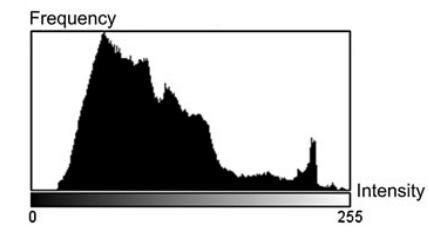
\includegraphics[width=0.5\textwidth]{8Misc/Pictures/Introduction/histogram_example.jpg}
	\caption{An example of a histogram. Image from \citep[ Chapter~4.3]{book:Moeslund}}
	\label{fig:HistogramEx}
\end{figure}

While it is possible using a histogram to detect several features of an image, it should be noticed that it is not possible to reconstruct an image based from a histogram. Thereby, it is also possible for several images to have the same histogram \citep{book:Moeslund}. \\

Histograms have so far been described as a tool to recognize distinct features of an image, but they can also be processed such that it can be used as an image manipulation tool - a term known as histogram processing. There exist different types of histogram processing regarding the type of operation needed. In the next section, some types of histogram processing have been described. \\

\textbf{Histogram stretching} \\
If the contrast is too low, the image might appear gray and unclear for humans. The characteristic of an image with low contrast is a narrow difference of gray-level intensity which is shown in the corresponding histogram of the image. An example of a gray-scale image with low contrast is shown in figure \ref{fig:HistogramLowContrast}. 

\begin{figure}[H]
	\centering
	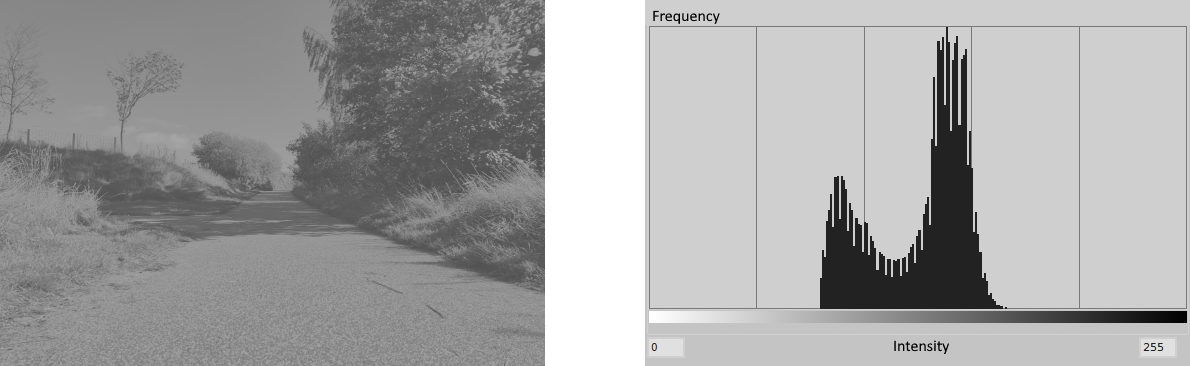
\includegraphics[width=1\textwidth]{8Misc/Pictures/Introduction/img_lc_full.jpg}
	\caption{Low contrast image with corresponding histogram}
	\label{fig:HistogramLowContrast}
\end{figure}

A solution for this problem is to map the gray-level values into an other value such that the level of gray-level intensities are spread out, which improves the contrast. This method is known as histogram stretching. Based on the original image shown in figure \ref{fig:HistogramLowContrast}, histogram stretching has been used to improve the contrast as shown in figure \ref{fig:HistogramImprovedContrast}.

\begin{figure}[H]
	\centering
	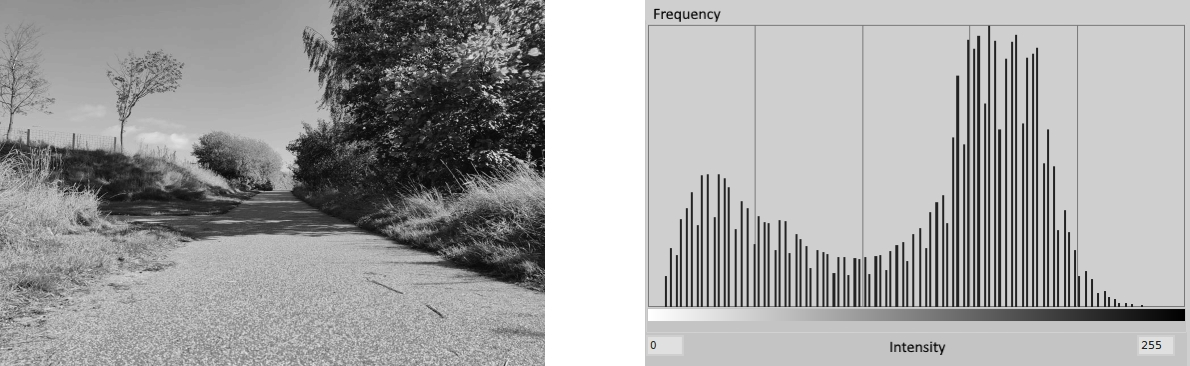
\includegraphics[width=1\textwidth]{8Misc/Pictures/Introduction/img_hc_full.jpg}
	\caption{Improved contrast image from figure \ref{fig:HistogramLowContrast} with corresponding histogram}
	\label{fig:HistogramImprovedContrast}
\end{figure}

\subsubsection*{Thresholding}
An other distinct feature for image processing is the ability to segment the image into several parts such as foreground with an object and background. While segmentation of an image is rather image analysis instead of image manipulation, it contains the necessary features for future image manipulation. Ideally, the segmentation between the background and object is visualized as a histogram with two significant peaks shown in figure \ref{fig:IdealHistogramThreshold}. A histogram with those characteristics is bi-modal. 

\begin{figure}[H]
	\centering
	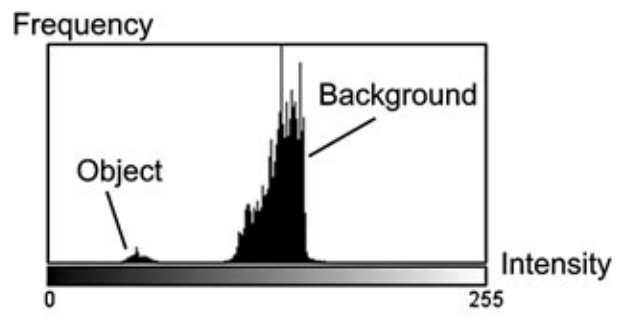
\includegraphics[width=0.5\textwidth]{8Misc/Pictures/Introduction/moeslund2012histogramThres.jpg}
	\caption{Ideal histogram \citep[ Chapter~4.4]{book:Moeslund}}
	\label{fig:IdealHistogramThreshold}
\end{figure}

In figure \ref{fig:IdealHistogramThreshold}, the peaks of object and background are clearly distinct from each other. However, it is generally difficult to distinguish objects from backgrounds due to the image containing a significant amount of information such as noise. One method of segmenting an image by reducing the amount of information is thresholding. \\

In thresholding, a threshold value $T$ is given. If the pixel value of an input image is under or equal to the threshold value, it will be mapped to the intensity value 0 - which is shown as black. All pixel values above the threshold value will be mapped to 255 (white). The advantage of using the thresholding method is that the object and background will be distinguished as black and white respectively. For an 8-bit input image $f(x,y)$, output image $g(x,y)$ and the given threshold value $T$, the algorithm can be described as the following equation \ref{eq:thresholdAlgorithm}:
\begin{equation}
\begin{aligned}
\text{if } & f(x,y) &\leq & \text{ } T & \text{then } & g(x,y) = 0 \\   
\text{if } & f(x,y) & > & \text{ } T & \text{then } & g(x,y) = 255
\end{aligned}
\label{eq:thresholdAlgorithm}
\end{equation}

During the process, some of the image's information will be lost or discarded, but the lost information is generally noise or otherwise redundant \citep{book:Moeslund}. \\

An example of using thresholding is shown in figure \ref{fig:ThresholdExample1} and \ref{fig:ThresholdExample2}.

\begin{figure}[H]
	\centering
	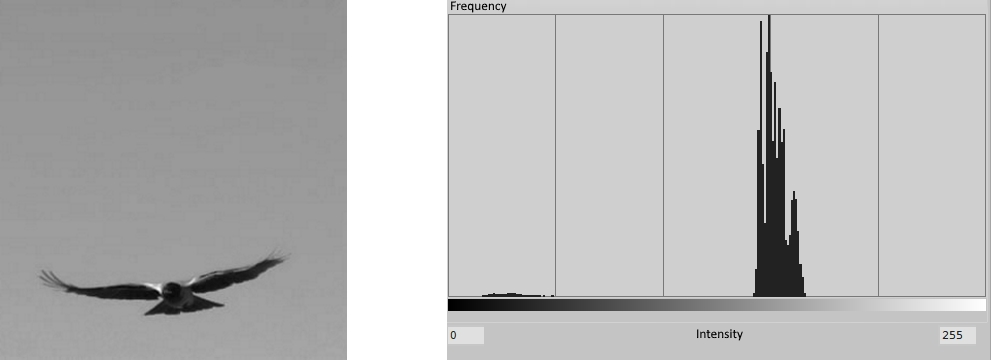
\includegraphics[width=1\textwidth]{8Misc/Pictures/Introduction/img_threshold_1.jpg}
	\caption{Gray-scale image with corresponding histogram}
	\label{fig:ThresholdExample1}
\end{figure}

The desired object in figure \ref{fig:ThresholdExample1} is the bird, while the background is the sky. In the histogram, a significant peak is shown at an intensity value of around 150. This indicates the background. However, a small peak is shown at the intensity value interval of around 25 to 60. This indicates the object as previously described and shown in figure \ref{fig:IdealHistogramThreshold}. Thereby, it is not necessary to segment the image using the thresholding method, however, it has been performed and shown in figure \ref{fig:ThresholdExample2} for further analyzing. 

\begin{figure}[H]
     \centering
     \begin{subfigure}[b]{0.3\textwidth}
         \centering
         
\includegraphics[width=1\textwidth]{8Misc/Pictures/Introduction/img_threshold_p0.jpg}
         \caption{$T = 0$}
         \label{subfig:ThresholdExample2_p1}
     \end{subfigure}
     \hfill
     \begin{subfigure}[b]{0.3\textwidth}
         \centering
         
\includegraphics[width=1\textwidth]{8Misc/Pictures/Introduction/img_threshold_p1.jpg}
         \caption{$T = 45$}
         \label{subfig:ThresholdExample2_p2}
     \end{subfigure}
     \hfill
     \begin{subfigure}[b]{0.3\textwidth}
         \centering
         
\includegraphics[width=1\textwidth]{8Misc/Pictures/Introduction/img_threshold_p2.jpg}
         \caption{$T = 127$}
         \label{subfig:ThresholdExample2_p3}
     \end{subfigure}
     \hfill
     \begin{subfigure}[b]{0.3\textwidth}
         \centering
         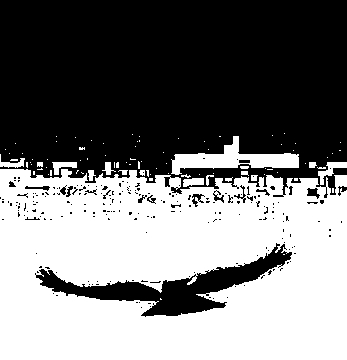
\includegraphics[width=1\textwidth]{8Misc/Pictures/Introduction/img_threshold_p3.jpg}
         \caption{$T = 150$}
         \label{subfig:ThresholdExample2_p4}
     \end{subfigure}
     \hfill
     \begin{subfigure}[b]{0.3\textwidth}
         \centering
         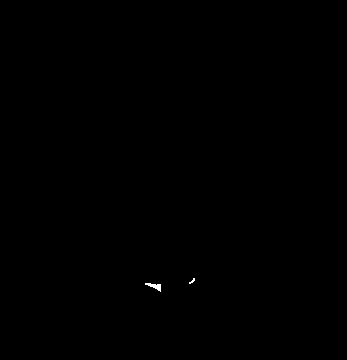
\includegraphics[width=1\textwidth]{8Misc/Pictures/Introduction/img_threshold_p4.jpg}
         \caption{$T = 200$}
         \label{subfig:ThresholdExample2_p5}
     \end{subfigure}
     \hfill
     \begin{subfigure}[b]{0.3\textwidth}
         \centering
         
\includegraphics[width=1\textwidth]{8Misc/Pictures/Introduction/img_threshold_p5.jpg}
         \caption{$T = 255$}
         \label{subfig:ThresholdExample2_p6}
     \end{subfigure}
    \caption{Image from figure \ref{fig:ThresholdExample1} with different threshold values}
    \label{fig:ThresholdExample2}
\end{figure}

Based on the histogram shown in figure \ref{fig:ThresholdExample1} and equation \ref{eq:thresholdAlgorithm}, it is seen in figure \ref{subfig:ThresholdExample2_p2} that most of the pixels for the object have an intensity value $T$ under 45. Due to this, those pixels are mapped to 0 and are shown in the image as black. If the threshold value is increased to 127, it is seen in figure \ref{subfig:ThresholdExample2_p3} that there is now an almost complete silhouette of the bird. However, looking at the histogram in figure \ref{fig:ThresholdExample1}, if $T$ is increased more, then $T$ would be greater or equal to the intensity values of the background. This is mostly shown in figure \ref{subfig:ThresholdExample2_p4} and \ref{subfig:ThresholdExample2_p5}, where in the first mentioned, parts of the background pixels are now being mapped to black and in the latter, almost the entire background has been mapped to black. \\

It is therefore important to find a good threshold value, where it is only the object and the background that is shown and segmented. Based on the example shown in figure \ref{fig:ThresholdExample1} and \ref{fig:ThresholdExample2}, it is seen that in figure \ref{subfig:ThresholdExample2_p4}, the silhouette of the bird is well-defined compared to figure \ref{subfig:ThresholdExample2_p3}, however, a significant portion of the background is mapped to black. Therefore, figure \ref{subfig:ThresholdExample2_p3} is more suitable for image processing in that case with a clear distinction between object and background. It can therefore be concluded that a good threshold value generally lies in the interval between the peak of the object and the peak of the background as shown in figure \ref{fig:ThresholdExample1}. \\

% WIP: Otsu method(?)

\subsubsection*{File format}
Finally, an other important factor in image processing is the size of the image file. A raw digital image contains all data from the image sensor, which means that this type of image files have high quality in regards to details, but will naturally also take up significant memory and storage. This image file is advantageous for editing/manipulating photos, when a very high quality photo is desired. However, for a real-time system, e.g. a surveillance system like a security camera, the bigger file sizes and longer processing times is significantly disadvantageous. For systems, where a smaller file size or faster processing times are needed, it is preferable to compress the image. There exists two types of compression: Lossless and lossy compression. \\

In lossless compression, the data is compressed such that the original data can be be perfectly reconstructed from the compressed data. Thereby, despite that the file size has been reduced due to the compression, no data has been lost. The compression has been done using several algorithms such as Huffman coding \citep{Lossless49:online}. In comparison to lossless compression, lossy compression focuses on minimizing the file size by removing redundant information. Therefore, some data might get lost in the process, which mean that the original image cannot be reconstructed perfectly based on the lossy compressed data. However, the compression algorithm has been optimized from the human vision's point of view, such that the compressed image looks very similar to the original. Compared to lossless compression, lossy compression is very efficient regarding the file size, where the compressed image's file size can be as small as 10\% of the original size without visible degradation of the image quality \citep{LossyDat32:online}. In table \ref{tab:ProConsFileFormat}, the different compression types are compared and their respective advantages and disadvantages have been highlighted. The disadvantages are taken from the point of view of image processing. Here, the preferable outcome is to have a small file size (thereby an efficient compressed image) that do not have any redundant data in the image. 

\begin{table}[H]
\centering
\begin{tabular}{ | p{2.85cm} | p{5.1cm} | p{3.3cm} | p{2.0cm} | }
\hline
\rowcolor{gray!25}
\textbf{Compression type}       & \textbf{Advantage}                                  & \textbf{Disadvantage}              & \textbf{Example of file type}         \\ \hline
No compression                  & Image of highest quality                      &  Big file size            &  .pgm, .ciff                          \\ 
(Raw)                           &                                               &  Long processing time     &                                       \\ \hline
Lossless                        & High quality image with smaller file size     &  Unnecessary data         &  .png, .gif                           \\ \hline
Lossy                           & Decent quality image with significantly smaller file size     & Heavy compression might degrade the image quailty  & .jpeg  \\
                                & Minimal-to-none redundant data                &                           &                                       \\ \hline                                              
\end{tabular}%
\caption{The advantage and disadvantage of different compression types}
\label{tab:ProConsFileFormat}
\end{table}


\subsection{Edge detection}
Edge detection is the process of finding the boundary of an object, meaning that in almost all cases, edges will represent the object in the image. The edge of an object can then be used to get a higher level of abstraction of the image, which means that the information in the image will be less thus easier to process. Before it is possible to find the edge of an image it is important to define what it is. Using a gray-scale image as a baseline it is possible to define an edge as a position where a significant change in gray-level takes place. Looking at figure \ref{fig: edge_pixel} on the left there is shown an image. To find an edge on that image a slice of that image can be taken vertically that is one pixel wide, which is illustrated in the figure between the arrows. By using this slice, a graph can be made where we can interpret the intensity value in the slice as the height in the graph that is shown on the right of figure \ref{fig: edge_pixel}. When looking at the graph when there is a significant change in the gray-scale value in the slice, the graph will also have a significant change in the height. These significant changes in the height is illustrated as circles in the graph, and is where the edges is defined in an image \citep[ Chapter~5.2.2]{book:Moeslund}.

\begin{figure}[H]  %(alternativt [H])
	\centering
	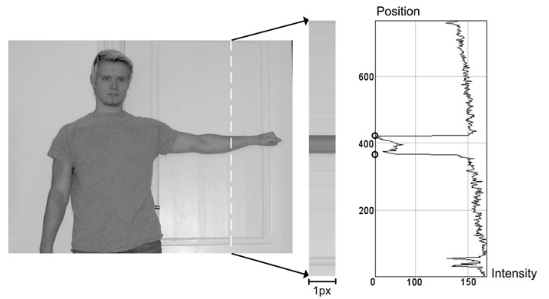
\includegraphics[width=1\textwidth]{8Misc/Pictures/Introduction/edge_pixel.png}
	\caption{A single column of the image is enlarged and presented in a graph. This graph contains
two very significant changes in height, the position of which is marked with circles on the graph.
This is how edges are defined in an image. Image from \citep[ Chapter~5.2.2]{book:Moeslund}}
	\label{fig: edge_pixel}
\end{figure}

To detect edges in an image the directional change in the intensity can be used, this concept is gradient in image processing. This can be done by representing the previous image in a 3D graph as seen in figure \ref{fig: edge_3d}. In the graph it is shown that the width and height of the image is represented by the x- and y-direction respectively, whereas the z-direction is represented by the intensity of the image interpreting it as height. 

\begin{figure}[H]  %(alternativt [H])
	\centering
	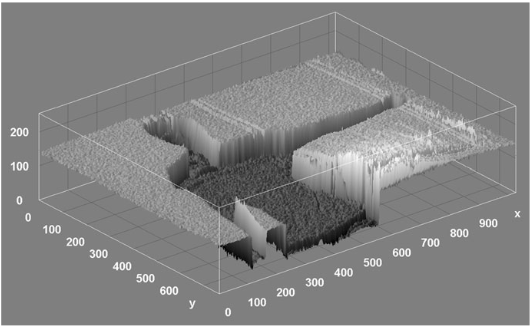
\includegraphics[width=1\textwidth]{8Misc/Pictures/Introduction/edge_3d.png}
	\caption{A 3D representation of the image from figure \ref{fig: edge_pixel}, where the intensity of each pixel is interpreted as a height. Image from \citep[ Chapter~5.2.2]{book:Moeslund}}
	\label{fig: edge_3d}
\end{figure}

For each point in the image there would be two partial gradients that would span a plane in the x- and y-directions intersecting a chosen point. These partial gradients can be used to determine the direction of the edge, as well as using their derivatives to calculate the resulting gradient by using eq. \ref{eq:Gradient}

\begin{equation} \label{eq:Gradient}
    \overrightarrow{G}(g_x , g_y)=\begin{pmatrix}
    g_x\\[\jot]
    g_y
    \end{pmatrix}=\begin{pmatrix}
    \frac{\partial f}{\partial x}\\[\jot]
    \frac{\partial f}{\partial y}
    \end{pmatrix}
\end{equation}

A gradient also has a magnitude, which is how steep the change of height is in the direction of the gradient and is also the length of the gradient vector. The length of the gradient vector can be calculated using the Pythagorean theorem solved for magnitude as seen in eq. \ref{eq:magnitude}
\begin{equation} \label{eq:magnitude}
    Magnitude^2 = g_x^2 + g_y^2 \Leftrightarrow Magnitude = \sqrt{g_x^2 + g_y^2}
\end{equation}
For faster implementation the magnitude can be approximated by using eq. \ref{eq:apmag}
\begin{equation} \label{eq:apmag}
    Magnitude = \abs{g_x} + \abs{g_y}
\end{equation}

As the partial gradients are first order derivatives it can not be calculated because an image is not a continuous curve and therefore needs an approximation. To calculate the approximation of the gradient it is possible to use the difference between the previous and next value seen in eq. \ref{eq:apgrad}

\begin{subequations}
    \label{eq:apgrad}
    \begin{align}
    g_x(x, y) \approx f(x+1, y) - f(x-1, y) \label{eq:xapgrad} \\
    g_y(x, y) \approx f(x, y+1) - f(x, y-1) \label{eq:yapgrad}
    \end{align}
\end{subequations}

This approximation will result in a gradient value that is positive when the pixel change from dark to bright and negative when it is reverse. It is possible to get the opposite value by switching the signs seen in eq. \ref{eq:opapgrad}
\begin{subequations}
    \label{eq:opapgrad}
    \begin{align}
    g_x(x, y) \approx f(x-1, y) - f(x+1, y) \label{eq:xopapgrad} \\
    g_y(x, y) \approx f(x, y-1) - f(x, y+1) \label{eq:yopapgrad}
    \end{align}
\end{subequations}

Equation \ref{eq:apgrad} can be applied with a 2D kernel using correlation, a 2D kernel is used because a 1 dimensional kernel is too sensitive to noise. A popular 2D kernel that is used is the Sobel kernel where the center pixel is weighed more which can be seen in figure \ref{fig: sobel}

\begin{figure}[H]  %(alternativt [H])
	\centering
	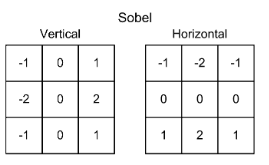
\includegraphics[width=0.4\textwidth]{8Misc/Pictures/Introduction/Sobel.png}
	\caption{A Sobel kernel. Image from \citep[ Chapter~5.2.2]{book:Moeslund}}
	\label{fig: sobel}
\end{figure}

What happens when using the sobel kernel is that the coefficients multiply the corresponding values around the source pixel then adding them together to get a sum of the values. This value will be a negative number if it goes from a bright to dark or in other words a bigger number to smaller number, in the other spectrum if it goes from a smaller number to a bigger number it will be a positive number. In the cases where the pixels are uniform the number given will be 0. This process where you calculate the sum can be seen in figure \ref{fig: convolve}

\begin{figure}[H]  %(alternativt [H])
	\centering
	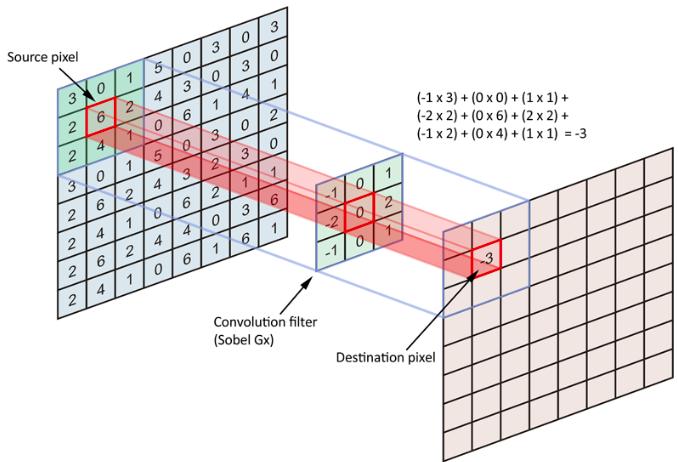
\includegraphics[width=0.8\textwidth]{8Misc/Pictures/Introduction/Sobel convolution.png}
	\caption{Sobel kernel calculation of convolution. Image from \citep{Medium}}
	\label{fig: convolve}
\end{figure}

It is possible to use the sobel kernel by combining the vertical and horizontal correlated images and then binarize the resulting image by thresholding it, but a better solution is to use the canny edge detector. The canny edge detector is an algorithm that uses the sobel kernel and also gives pixel-thin edges, this process is done in 5 steps:
\begin{enumerate}
    \item Apply a Gaussian filter to smooth the image and remove noise
    \item Find the gradients using the sobel kernel 
    \item Apply non-maximal suppression, by comparing a pixel with its neighbors in the gradient direction
    \item Apply double threshold comprising of $T_{high}$ and $T_{low}$
    \item Categorize an edge that is localized higher than $T_{high}$ as a strong edge and as weak edge if between $T_{high}$ and $T_{low}$, then only keep edges that are strong or connected to a strong edge
\end{enumerate}

\begin{figure}[H]  %(alternativt [H])
	\centering
	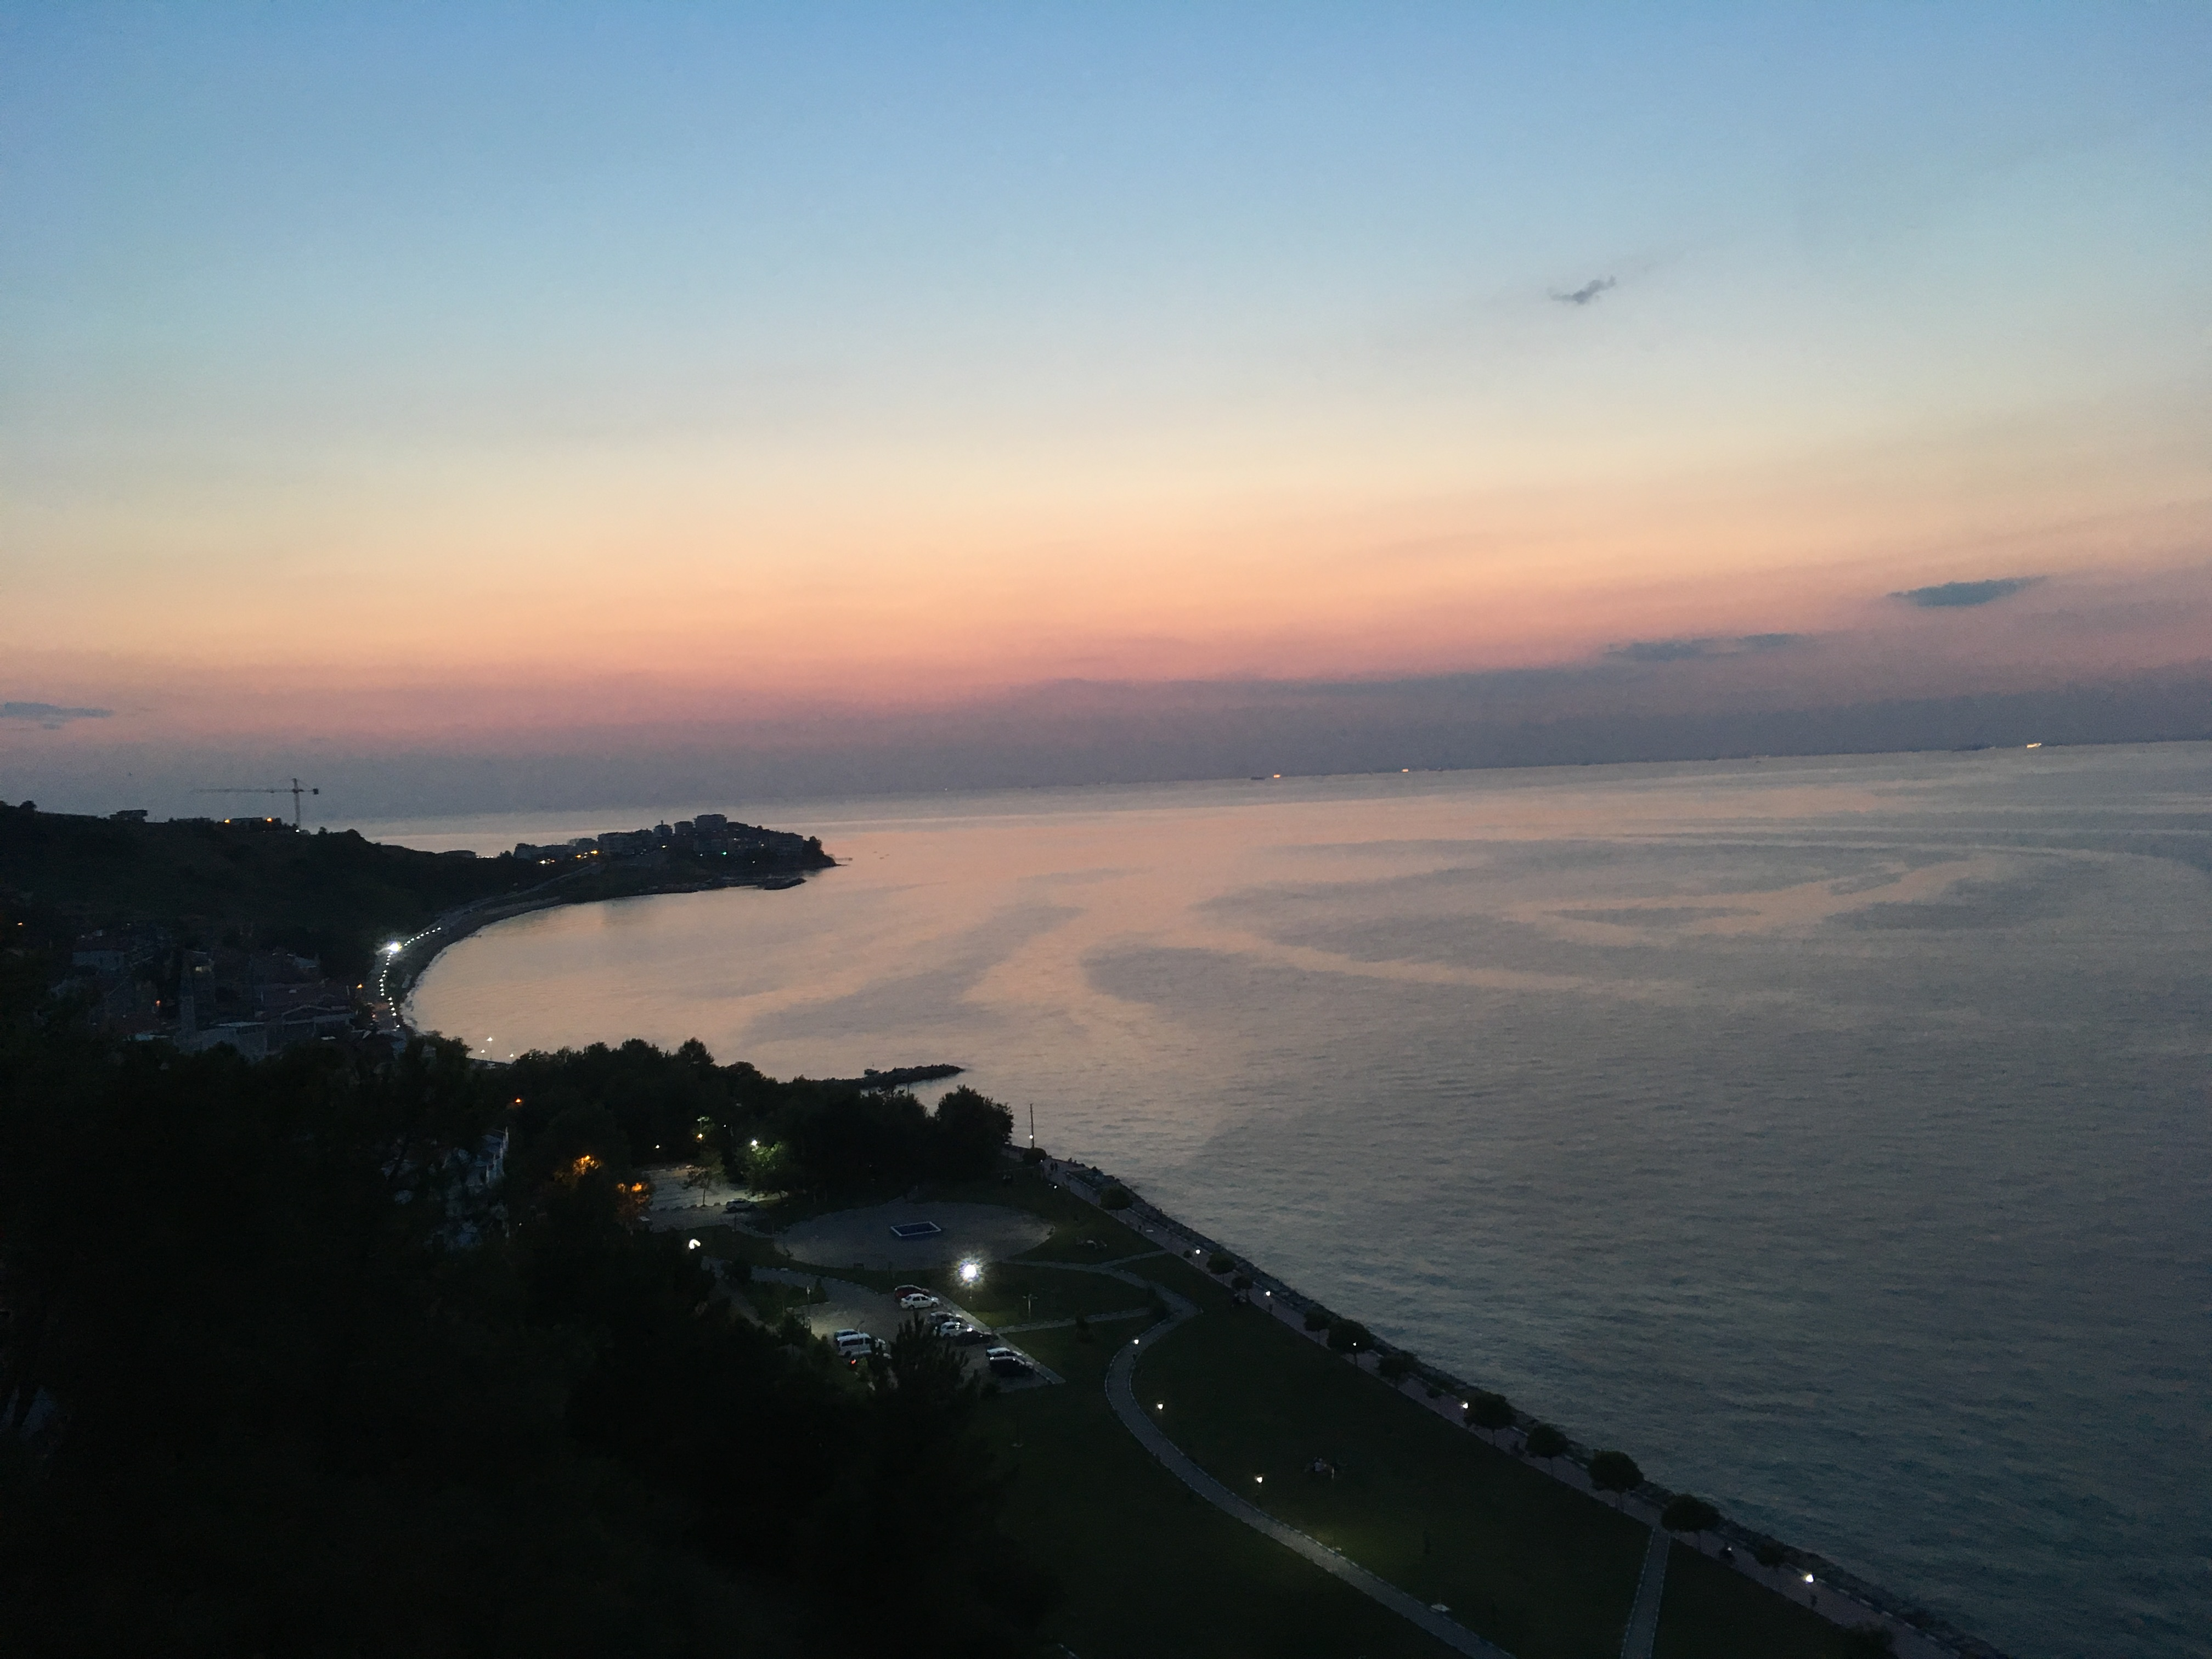
\includegraphics[width=1\textwidth]{8Misc/Pictures/Introduction/land.JPG}
	\caption{original}
	\label{fig: convolve2}
\end{figure}

\begin{figure}[H]  %(alternativt [H])
	\centering
	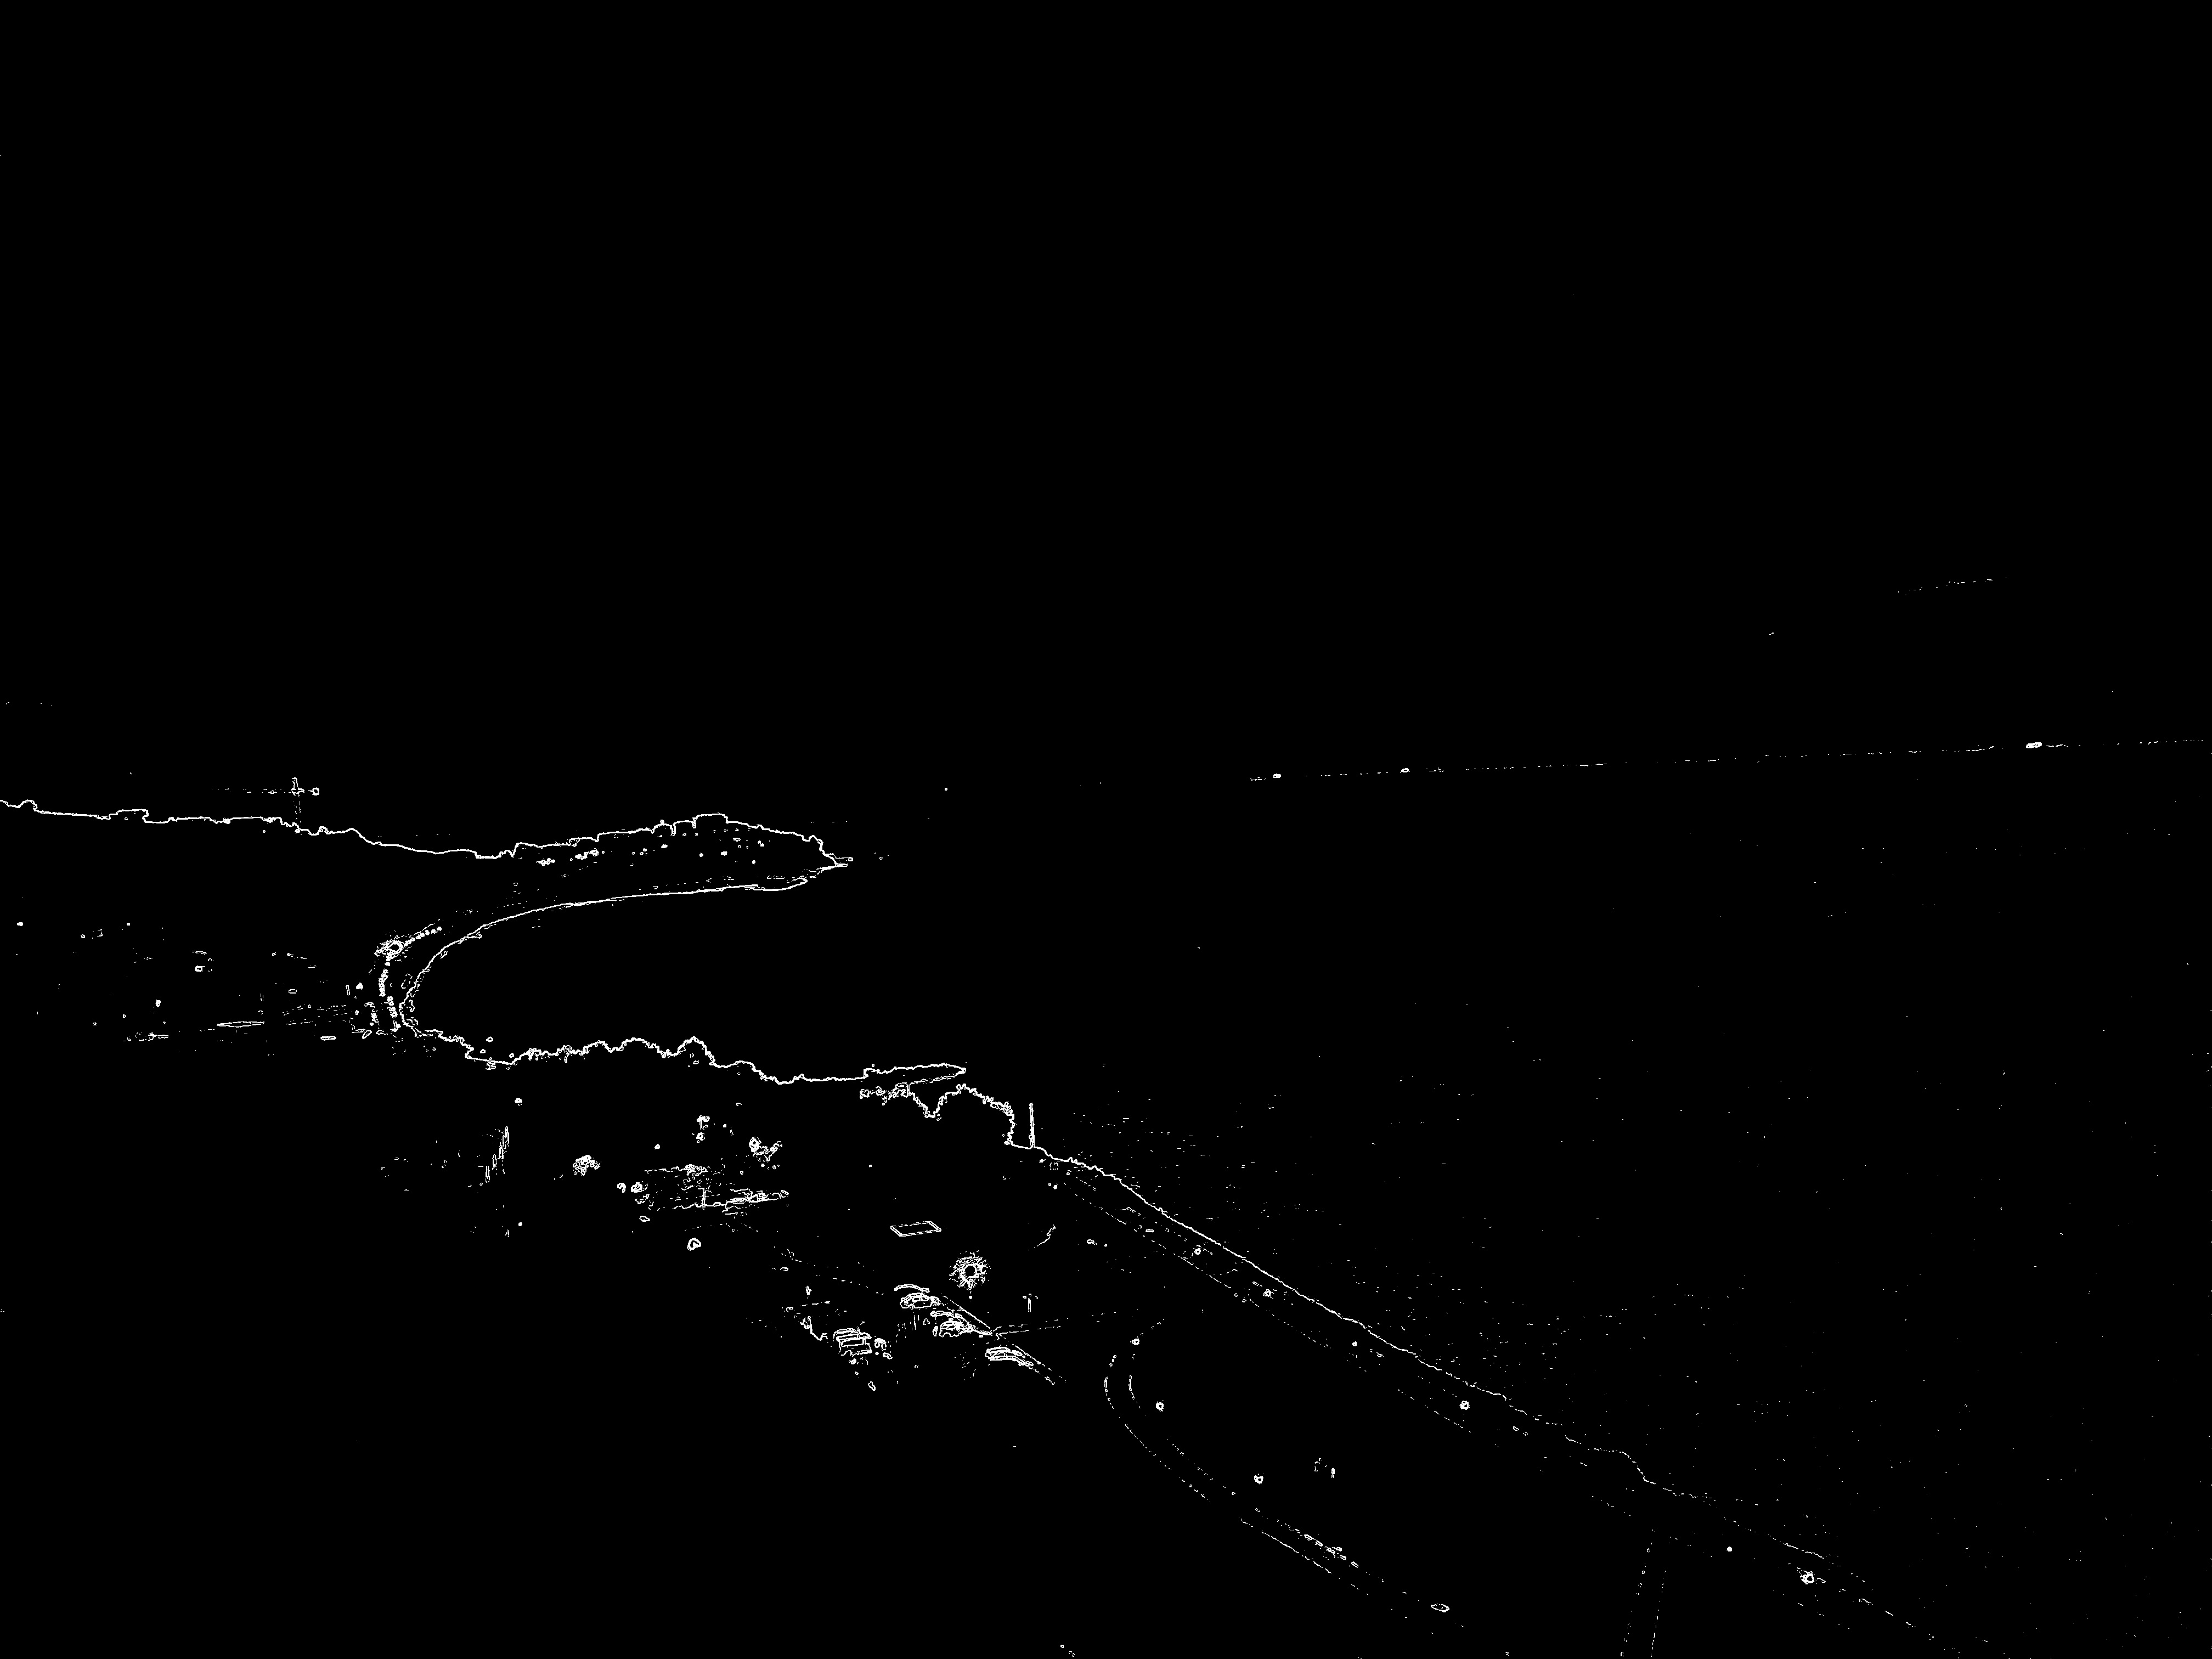
\includegraphics[width=1\textwidth]{8Misc/Pictures/Introduction/landsobel.JPG}
	\caption{Sobel}
	\label{fig: convolve3}
\end{figure}

\begin{figure}[H]  %(alternativt [H])
	\centering
	
\includegraphics[width=1\textwidth]{8Misc/Pictures/Introduction/landcanny.JPG}
	\caption{Canny}
	\label{fig: convolve4}
\end{figure}

%sobel

%canny





\section{Environment}

\section{RFID}
lknasdfsdlkndsakndlksna

\section{Cage}

\section{Noise}

\section{Scenario}
% (Ud fra problemanalysen) Hvilke objekter (el. aktører) har vi med at gøre? forklar hvad det hvad det gør osv
% forklar vores use case hvad skal der ske. (det skal lave en historie som giver diagrammet) 
% use case diagram

To solve the problem statement, the system needs a means to detect a cage, to identify the cage, to observe the movement of said cage, to analyze these observations and to store the resulting information. To detect, and identify the cage an RFID sensor is a functional solution. It will register the cage and it's associated ID when the cage is within range. To observe it, a camera will be utilized. This will stream the movements of the cage to the processing device. To process this data, a PC or a specialized device is required to do the heavy lifting. A database will be used to store the results of the analysis, along with the RFID tag that is associated.

\begin{enumerate}
    \item The system can start only when the RFID sensor has detected the cage is in range and then get the cages ID, which can the be stored
    \item After the cage has been detected the camera can start streaming the video and the movement of the cage.
    \item With the streaming data the footage can be processed by a computer in real or near real time to identify the cage and detect the direction of the cage.
    \item When the direction of the cage has been found it can then be sent, along with the cages ID, to a database which then can be stored for easy access and readability.
\end{enumerate}

From the presented scenario, an overview of the systems functionalities can be outlined. This is done by a use case diagram where the actors are the PC (Computer), the RFID sensor, the camera, and the database where the primary actor is the PC. The use case diagram is shown in figure \ref{fig:UseCase_CageMovement}

\begin{figure}[H]  %(alternativt [H])
	\centering
	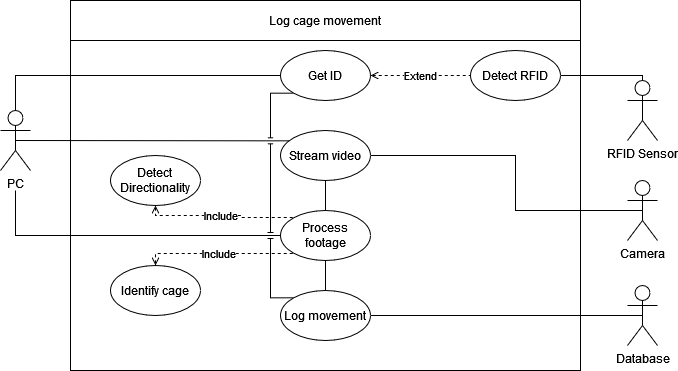
\includegraphics[width=1\textwidth]{8Misc/Pictures/Introduction/Use case.png}
	\caption{Use Case}
	\label{fig:UseCase_CageMovement}
\end{figure}

%%%%% DISPOSITION %%%%%

    % Camera  - Winter
        % Basics of Cameras
            % Light
                % Electromagnetic waves
            % Image acquisition

        % Camera properties
            % Focus
            % FoV
                % Concave vs convex lenses
            % Aperture 
            % Shutterspeed
            % Zoom
            % ISO
            
        % Data properties
            % Bayer pattern
            % Contrast
                % Quantization
                
            % Color
                % Magenta isn't real
                % RGB to HSI< conversion
                % HSI, HSV

    % Image Processing
        % Introduction 
            % Digital image structure
            % Digital color theory

        % Data interpretation and manipulation - Khadar (until thresholding)
            % File format
            % Pixel representation
            % Histogram (relevant??)
            % Thresholding
                % Otsu method
            %Correlation
                % Filters
                    % Median/mean/rank
                    % pattern recognition
            % Morphology
                %Structure element
                % zero/Null
                % Hit (Dilation)
                % Fit (Erosion)
                % Multiple operations
                    % Opening
                    % Closing
            % Blob Detection
                % BLOB!
                % Connected component analysis
                    % Grassfire algorithm
                        % 4 and 8 connectivity
                        %Iterative and recursive
                            % Burn Queue
                    % Region growing
                    % Feature extraction
                    % Feature matching
            
        % Edge detection (steps + methods) - Kazim
            % Sobel edge detection
            % Canny edge detection
            
        % Computer Vision and Machine learning
            % OpenCV
            % TensorFlow
            
    
            
    
    % Environment

    % RFID
        % Antenna
        % Tags
        % 96 bit
        % Aktiv
            % Exciter scenario
        % Passiv
        % Phasing

    % Cage
        % Dimensions
        % Shape

    % Background Noise
        % Light pollution
        % Radio pollution
            % Excess objects
                % Humans
                % Trucklift
                % Machines
                % Packages
    
    % Scenarios
        % Objects
        % Use cases
        % Use case diagram
            
                
        

% Problem specification (what is the problem) (different chapter)
    % Usage of cameras (how many cameras do we need to solve the problem?)

    % System specification 
        % Accepttests


% Unsorted things
    % Tile image to determine movement (possible solution)
    % Angle of incidence
\chapter{Design}


\chapter{Implementation}


\chapter{Tests}


\chapter{Discussion}



\chapter{Conclusion}



%%%% Kilder %%%%

\begingroup
	\raggedright
	\bibliography{7Formalia/literature}
\endgroup


%%%% Fixme-listen %%%%

\newpage														% Ny side til Fixme-listen
\listoffixmes	
% Fixme-listen - fjernes til sidst i projektet med "%"
%\listoftodos

%%%% Appendiks %%%%

\appendix														% Appendiks/bilag start - giver chapter bogstaver i stedet for tal
\clearforchapter												% Sikrer at pagestylen aktiveres paa den rigtige side
\phantomsection													% Kunstigt afsnit, som hyperlinks kan 'holde fast i'
\pdfbookmark[0]{Appendiks}{appendiks}							% Tildeler en klikbar bookmark til den endelige PDF

%% Indstillinger for appendiks (deaktiveret med "%") %%

%\pagestyle{empty}												% Sidehoved/-fod for standardsider aendres til tom for appendiks
%\aliaspagestyle{chapter}{empty}								% Sidehoved/-fod for kapitelsider aendres til tom for appendiks
%\settocdepth{chapter}											% Kun kapitel-niveau vises i ToC
%\addtocontents{toc}{\protect\cftpagenumbersoff{chapter}}		% Sidetal for kapitler fjernes i ToC

%% Filer til appendiks %%

%\chapter{Appendix}



%%%% Bilag %%%%

%\phantomsection												% Kunstigt afsnit, som hyperlinks kan 'holde fast i'
%\addcontentsline{toc}{chapter}{Bilag A \ Navn} 				% Manuelle indgange i indholdsfortegnelsen (naar \includepdf bruges)

%\includepdf[pages={x-y}]{filnavn}								% Inkluder eksterne bilag med \includepdf[pages={x-y}]{filnavn}


\end{document}													% Slutter dokumentet - obligatorisk


